%----------------------------------------------------------------------------------------------------------------------

\documentclass[a4paper,12pt]{report}
\usepackage[utf8]{inputenc}
\usepackage[portuguese]{babel}
\usepackage{graphicx}
\usepackage{hyperref}
\usepackage{float}
\usepackage{listings}
\usepackage{longtable}
\usepackage{subfig}
\usepackage{tabularx}
\usepackage[table,xcdraw]{xcolor}
\usepackage{adjustbox}
\newcommand*{\xml}[1]{\texttt{<#1>}}
\usepackage[T1]{fontenc}
\usepackage{lmodern}
\newcommand*{\escape}[1]{\texttt{\textbackslash#1}}
\newcommand*{\escapeI}[1]{\texttt{\expandafter\string\csname #1\endcsname}}
\newcommand*{\escapeII}[1]{\texttt{\char`\\#1}}
\usepackage[bottom]{footmisc}

%----------------------------------------------------------------------------------------------------------------------

\usepackage{geometry}
 \geometry{
     a4paper,
     total={170mm,257mm},
     left=25mm,
     right=25mm,
     top=20mm,
 }

\graphicspath{{./base_images/}}

%----------------------------------------------------------------------------------------------------------------------

\begin{document}

%----------------------------------------------------------------------------------------------------------------------


\begin{titlepage}
    \center
    {

    \begin{figure}[t]
        \centering
        
\includegraphics[scale=0.4]{images/uminho.png}
        \label{img:logo}
        \vspace{2.0cm}
    \end{figure}

    \vspace{3.0cm}
    \textsc{\Huge Processamento de Linguagens}\\[0.5cm]
    \textsc{\Large{Mestrado Integrado em Engenharia Informática}}\\[0.5cm]
    \vspace{3cm}
    \textsc{\huge{Conversor de TOML para JSON}}\\[1cm]
    \textsc{\large{[YACC/FLex]}}\\[0.5cm]
    \vspace{4cm}
    \begin{flushleft}

        \vspace{1cm}
        \large 
        \vspace{0.5cm}

        \large A85227 \,\,\,João Pedro Rodrigues Azevedo
        \vspace{0.2cm}

        A85729 \,\,\,Paulo Jorge da Silva Araújo
        \vspace{0.2cm}

        A83719 \,\,\,Pedro Filipe Costa Machado
        \vspace{0.2cm}

    \end{flushleft}
    \begin{flushright}
        Braga

        Junho 2020
    \end{flushright}

\date{\today}
}
\end{titlepage}

%Indice

\tableofcontents
\clearpage

% Introdução

\chapter{Introdução}

Este relatório é relativo ao segundo trabalho prático da UC de Processamento de Linguagens que tem como um dos principais objetivos escrever gramáticas independentes de contexto (GIC) que satisfaçam a condição LR(), para criar Linguagens de Domínio Específico (DSL).
\par
Para tal, iremos recorrer a geradores de compiladores como o par \textbf{FLex/Yacc} e ainda desenvolver processadores de linguagens regulares capazes de alterarem e transformarem textos segundo o método da tradução dirigida pela sintaxe, suportado numa gramática tradutora (GT).
\par
Este trabalho serve também como a introdução e aplicação de linguagens de programação como o \textbf{TOML} e o \textbf{JSON} na leitura e representação final dos dados obtidos após reconhecimento de frases válidas da nossa linguagem.

\chapter{Enunciado Escolhido}

Como pedido pela equipa docente, para a escolha do enunciado para a realização deste projeto usamos a fórmula \textit{exe = (NGr \% 6) + 1} que aplicada ao nosso grupo (nº 69) resultou na escolha do enunciado quatro, um conversor \textbf{toml2json} (enunciado 2.4).
\par Desta forma, foi necessário proceder a uma breve pesquisa com intuito de percebermos o que é a linguagem \textbf{TOML} e de que forma se comporta, visto que nenhum dos elementos do grupo tinha trabalhado com este formato de arquivos. 
\par Percebemos então que o \textbf{TOML} é um formato de arquivo de configuração criado para ser mais legível para os humanos e que usa uma sintaxe mínima na representação de pares chave-valor.

\vspace{0.3cm}

\par Assim, de modo a cumprir os objetivos deste trabalho prático, devemos escolher um subconjunto de regras da linguagem \textbf{TOML} que o nosso conversor vai seguir. Neste relatório iremos indicar quais as regras que são possíveis de aplicar e como procedemos para a sua conversão em \textbf{JSON}.


\chapter{Estratégia Adotada}

\par Com vista a estudar a linguagem \textbf{TOML}, o \textit{website} disponibilizado pela equipa docente serviu para retirar informações precisas e claras sobre esta linguagem. \par Deste modo, podemos verificar todas as regras que são aplicadas no \textbf{TOML} e retirar exemplos para depois os aplicar ao nosso conversor, comparando o resultado com vários conversores \textit{online}.

\vspace{0.5cm}

\section{Gramática do TOML}

Tal como proposto, foi selecionado um subconjunto de regras da linguagem \textbf{TOML} a que nos comprometemos a aplicar e depois representar no \textbf{JSON} final.

\vspace{0.3cm}

\par A linguagem \textbf{TOML}, no nosso entender, pode ser representada através de um conjunto de tabelas e atribuições. Cada atribuição pode estar ``ligada'' a uma tabela, comportando-se como um atributo dela. Uma tabela, por sua vez, tem um número ilimitado de atribuições. Devido a este comportamento da gramática do \textbf{TOML}, a definição de tabelas, sub-tabelas e atribuições foram os principais focos para o subconjunto considerado.

\par Desta forma, iremos abordar os vários pontos na definição de uma linguagem \textbf{TOML}.

\vspace{10cm}

\subsection{Atribuição}

O \textbf{TOML} segue a prática de muitas outras linguagens no que toca à atribuição de valores e variáveis. Esta atribuição é caracterizada por uma \textbf{Key} e um \textbf{Value} da seguinte forma:

\vspace{0.5cm}

\par \textbf{Sintaxe: Key = Value}

\vspace{0.3cm}

\begin{itemize}
    \item \textbf{Key}
    \par Uma \textbf{Key} pode ser uma ou mais palavras, sendo que para usar várias é necessário colocá-las entre aspas ou plicas.
    \par Assim, pode-se colocar uma série de caracteres, pois o \textbf{TOML} não é restritivo nesse parâmetro. Contudo, os caracteres especiais não são permitidos sem a colocação de aspas/plicas.
    \begin{verbatim}
        Exemplos de Keys:
        "maçã", banana, tuti_fruta, "tomate é um fruto", ...
    \end{verbatim}
    \item \textbf{Value}
    \par Um \textbf{Value} pode assumir vários valores e serve para caracterizar a \textbf{Key} respetiva. 
    \par Neste conversor foram considerados quase todos os tipos de dados disponíveis no \textbf{TOML}, com a exceção das \textit{strings multi-line}, pois apenas se considerou as \textit{strings} clássicas com apenas uma linha, usando caracteres especiais como \escape{n}, \escape{t}, ...
    \begin{verbatim}
        Número: 3
        String: "morango"
        Boolean: true
        Date-Time: 1979-05-27T07:32:00
        Array: [1,2,3]
    \end{verbatim}
    \par As strings consideradas no nosso conversor são bastante simples, pelo que não é possível ter plicas ou outras aspas dentro destas.
    \par Destes \textit{values} há que destacar que os \textit{arrays} do \textbf{TOML} precisam de ter para todos elementos o mesmo tipo de variável, ou seja, algo como o seguinte \textbf{não é possível}:
    \begin{verbatim}
        array = [1, 2, true, "vermelho"]
    \end{verbatim}
    Sendo que um exemplo de \textit{array} válido, seria:
    \begin{verbatim}
        cores = ["verde", "amarelo", "vermelho",]
    \end{verbatim}
    A linguagem \textbf{TOML} aceita a vírgula no final, embora possa não estar presente. De realçar que também é possível obter \textit{arrays} de \textit{arrays}, sendo que cada elemento precisa de ser sempre um \textit{array}.
    \begin{verbatim}
animal = [ ["raposa", "cão"], ["camarão", "peixe-espada"], [1, 2] ]
    \end{verbatim}  
    
\end{itemize}  

\vspace{10cm}

\subsection{Tabelas}

\par As tabelas no \textbf{TOML} servem para agrupar dados de maneira simples. Assim, uma tabela pode ter várias atribuições referenciadas a ela própria através das atribuições ``filhas''. Contudo uma tabela nunca tem uma atribuição associada a ela mesma!
\par Na gramática de \textbf{TOML} uma atribuição está sempre referenciada à última tabela inicializada, ou seja, à tabela acima, caso exista. 

\begin{verbatim}
[morango] = "vermelho"   # Não é permitido!

[frutos]
morango = "vermelho"
\end{verbatim}

\par Neste exemplo, a \textbf{key} \textit{morango} está referenciada na tabela \textit{frutos} com o \textbf{value} \textit{``vermelho''}.

\vspace{0.3cm}

As tabelas em \textbf{TOML} podem ser definidas através do uso dos parênteses retos (``['' e ``]'') como se observa no exemplo anterior. Dentro dos parênteses retos aceitam-se palavras com ou sem aspas, pelo que as últimas não podem ser do tipo ``'' (vazio), ou seja, precisam de conter pelo menos um caractere.

Para além desta definição simples de uma tabela, podemos definir um conjunto de tabelas com uma hierarquia através do ponto:
\begin{verbatim}
    [frutos.morango]
    [frutos."maçã"]
    [frutos.laranja.casca]
\end{verbatim}

Aqui a tabela frutos tem várias tabelas ``filho'' (morango, ``maçã'' e laranja), sendo que a última também possui a referência para outra tabela.
\par Deste modo, é possível definir uma hierarquia de tabelas sendo que cada uma delas pode conter atributos e/ou outras tabelas.

\par Contudo, na definição das tabelas é preciso ter em consideração que o \textbf{TOML} não permite a definição da mesma tabela, ou seja, tabelas com o mesmo nome.

\begin{verbatim}
    [frutos]
    morango = "vermelho"
    [frutos]            # Não é permitido!
\end{verbatim}

\par A linguagem \textbf{TOML} também possui outra forma de inicialização de tabelas hierárquicas com uma atribuição que também foi tido em conta neste conversor:

\begin{verbatim}
    frutos."com caroço"."pêssego" = 2
    
    É equivalente a: 
    
    [frutos]
    [frutos."com caroço"]
    "pêssego" = 2
\end{verbatim}

Como podemos observar, temos duas maneiras diferentes de introduzir a hierarquia de tabelas. Neste exemplo, estamos a criar uma tabela \textit{frutos} com uma outra tabela \textit{``com caroço''} que possui uma atribuição.

\subsection{Comentários}

A linguagem \textbf{TOML} é muito semelhante a \textbf{JSON} e \textbf{YAML} visto que todas elas servem para descrever ficheiros de configuração de forma muito simples. \textbf{TOML} e \textbf{YAML} são muito semelhantes no que toca à simplicidade do ser humano em ler a linguagem, e, por isso mesmo, é possível adicionar comentários no ficheiro\footnote{O formato \textbf{JSON} não permite comentários, ao contrário de \textbf{TOML} e \textbf{YAML}}.

\vspace{0.3cm}

\par Os comentários em \textbf{TOML} são efetuados através do símbolo \#, que marca a linha após este como sendo um comentário.
\par Assim, o nosso conversor ignora qualquer informação na linha após o \#, excepto quando se encontra dentro de uma \textit{string}.

\begin{verbatim}
    [frutos]
    # A tabela em cima é para frutos
\end{verbatim}

\vspace{1cm}

\section{Analisador Léxico, FLex}

O analisador sintático gerado pelo \textbf{Yacc} requer um analisador léxico que é fornecido externamente através do \textbf{FLex} que habitualmente conhecemos, aplicado no primeiro trabalho prático.
\par
Assim, visto que o \textbf{Yacc} não lê a partir duma simples entrada de dados, temos a necessidade de implementar um analisador como o anterior para poder fornecer os \textit{tokens} necessários de modo a perceber a semântica introduzida.
\par
Por isto, tivemos que definir uma série de expressões regulares que identificam esses \textit{tokens}, seguindo-se uma breve descrição de alguns exemplos práticos aplicados no analisador léxico:
\par

\begin{enumerate}

    \item \textbf{Reconhecimento de números inteiros ou com vírgula flutuante:}
    
\begin{verbatim}
    Regex (números): [-+]?[0-9]*(\.)?[0-9]+([eE][-+]?[0-9]+)?
\end{verbatim}
\par
A expressão regular anterior permite o reconhecimento de números positivos ou negativos com vários algarismos e, inclusivé, introduz possibilidade de casas decimais e notação científica, por exemplo: \textbf{$1.02$}, \textbf{$-93$},  ou até \textbf{$94.93e-9$}.
\par
Posto isto, o \textit{token} retornado e previamente definido no \textbf{Yacc} é o \underline{\textbf{NUM}}, generalizando, assim, a introdução de \textit{integers} ou \textit{floats} por utilizadores.
\par O valor definido para esse número será guardado numa \textit{union} intercalada entre os programas onde o valor de \textit{yylval.number} é definido através da conversão da sequência de \textit{chars} reconhecida, \textbf{yytext}, para \textit{float}.

\vspace{5cm}

    \item \textbf{Reconhecimento de valores booleanos:}
    
\begin{verbatim}
    Regex (bools): (true|false)
\end{verbatim}

Os valores booleanos podem ser facilmente confundíveis com o reconhecimento de palavras pelo que são, por isto mesmo, palavras reservadas.\par
Deste modo, o \textit{token} enviado ao \textbf{Yacc} corresponde à \textit{macro} definida para \underline{\textbf{BOOL}} sendo, no entanto, guardado o seu valor como uma simples \textit{string} no campo \textit{yylval.string} da estrutura de dados partilhada.

    \item \textbf{Reconhecimento de datas:}
    
\begin{verbatim}
    Regex (datas): [0-9]+-[0-9]+-[0-9]+([T ][0-9]+\:          \\
                   [0-9]+\:[0-9]+(Z|([+-][0-9]+\:[0-9]+))?)?
\end{verbatim}

As datas são necessariamente uma sequência de caracteres mais comprida de reconhecer, pois seguem os padrões estabelecidos pelo \textbf{ISO 8601} para representações universais de datas na \textit{Internet}.\par
Esta expressão regular aceita assim exemplos como o seguinte:
\begin{verbatim}
Exemplo: 1994-11-05T08:15:30-05:00 
\end{verbatim}
Que corresponde a 5 de Novembro de 1994, 8h15m30s da manhã nos padrões "US Eastern Standard Time". Posto isto, o \textit{token} retornado é definido como \underline{\textbf{DATE}} e os \textit{chars} reconhecidos são armazenados no \textit{yylval.string} .

    \item \textbf{Reconhecimento de chaves (\textit{keys}) e \textit{strings}:}
    
O reconhecimento das variáveis que serviram de indexação e orientação na construção da estrutura de dados que viria a ser convertida para \textbf{JSON}, foi mais um desafio na realização deste trabalho prático.\par
Na prática, a introdução de chaves ou variáveis é relativamente simples considerando-as como uma sequência de caracteres como na seguinte expressão regular:

\begin{verbatim}
    Regex (chaves normais): [a-zA-Z_0-9-]+  
\end{verbatim}
\par
Onde o seu intuito é reconhecer o \textit{left-hand-side (lhs)} de uma atribuição (\textbf{a }= ...), a inicialização de tabelas ([a]) ou a construção de termos a partir da concatenação de várias chaves ([\textbf{a.b}] ou \textbf{a.b}). 
\par No entanto, a versatilidade do \textbf{TOML} faz com que sejam também permitidas como chave \textit{strings} (não vazias), pelo que os exemplos seguintes são também válidos:

\begin{verbatim}
"a" = 2  ou "b".c = 3 ou ["d"] ...
//Nota: "" = ... ou [""] são situações inválidas!
\end{verbatim}

Esta propriedade interessante levou-nos a introduzir uma nova expressão regular que teria necessariamente de fazer uma série de verificações relativamente ao reconhecimento de \textit{strings}, não esquecendo as possíveis situações de erro, tendo definido para isso um \textit{token} \underline{\textbf{ERRO}} não reconhecido pela gramática:

\begin{verbatim}
Regex (strings chaves ou valor): ["'][^'"=]*["']       
Ação: { 
        
        if (*yytext != *(yytext+strlen(yytext)-1)) 
            return (ERRO);
                          
        if (IS_RHS) 
        {
            yylval.string = strdup(yytext); 
            IS_RHS = 0;
            return (STRING);
        } 
        else 
        {
            if (strlen(yytext)==2) return (ERRO);
            yylval.string = strdup(yytext); 
            IS_RHS = 1;
            return (KEY_STRING);
        }
    }                
\end{verbatim}

Esta expressão regular tanto reconhece \textit{strings} como valores ou como chaves, sendo que, no caso de serem chaves estas têm necessariamente de ter tamanho superior a 2, ou seja, as duas aspas que lá estão sempre mais a \textit{string} em si.
\par
Em ambos os casos, a primeira verificação, isto é, o primeiro \textit{if} garante que o primeiro caractere reconhecido é igual ao último, ou seja, começa com aspa e termina com aspa e caso isso não se verifique envia-se ao \textbf{Yacc} o \textit{token} \underline{\textbf{ERRO}}.
\par
De seguida, definiu-se uma variável global ao programa,  \textbf{IS\_RHS} que serviria para identificar se estaríamos na fase de \textit{parsing} do lado esquerdo (valor = 0) ou lado direito (valor = 1) de uma atribuição, porque para o caso de \textit{IS\_RHS == 0} então estaríamos a reconhecer uma chave de uma atribuição (ou não) e esta não pode ser vazia (caso \textit{else}), retornando para esse caso um \textit{token} \underline{\textbf{KEY\_STRING}}. 
\par
Por outro lado, caso \textit{IS\_RHS == 1}, estamos no lado direito de uma atribuição e portanto a \textit{string} já pode ser vazia, retornando para esse caso um \textit{token} \underline{\textbf{STRING}}.

\par
Definir se estamos de um lado direito da atribuição é possível de se fazer no caso do reconhecimento do caractere \textbf{=} (e outros), já o caso do lado esquerdo estabelece-se quando estamos no \textit{rhs} e lemos uma valor ou quando encontramos caracteres como o \textbf{"."} associados a chaves:

\begin{verbatim}
Regex (atribuição, parenteses): [\[\]=,] { IS_RHS = 1; ... }
Regex (ponto, comentário): [.#] { IS_RHS = 0; ... }    
\end{verbatim}

    \item \textbf{Reconhecimento de outras expressões:}
    
    Obviamente, para além dos vários símbolos variáveis definidos anteriormente é necessário incluir o reconhecimento de sinais como o caractere do comentário (numa linha) e outros caracteres ignorados como o de mudança de linha, tabulação, etc...estabelecendo, por último, um caso \textit{otherwise} para todos os caracteres desconhecidos reconhecidos pelo \textbf{FLex}.

\end{enumerate}


\section{Analisador Sintático, Yacc} 

\par Após a implementação da parte léxica, tivemos de desenvolver o código do analisador sintático (\textbf{Yacc}) de forma a receber os símbolos provenientes do \textbf{FLex} e, a partir destes, verificar se cumpre a gramática pretendida, sendo neste caso um subconjunto da linguagem \textbf{TOML}.

\vspace{0.3cm}
O símbolo não terminal principal do nosso conversor chama-se de \underline{Toml} e deriva apenas em \underline{Language}. 
\par De seguida, o \underline{Language} pode resultar em \underline{Atributions} que representa uma lista de atribuições ou num \underline{Atributions} seguido do símbolo \underline{Declarations} onde se definem todas as declarações de tabelas. A razão pela qual o símbolo terminal \underline{Language} deriva nestas duas produções deve-se à possibilidade da ocorrência de atribuições não relacionadas a nenhuma tabela e a atribuições sempre relacionadas a tabelas\footnote{Caso tenhamos uma declaração no início, todas as atribuições seguintes são sempre referentes a uma tabela já definida.}. 
\par Desta forma, a primeira produção, visto que o \underline{Atributions} pode derivar em vazio, indica que podem haver apenas declarações ou atribuições (ou não caso seja vazio) seguidas de declarações. A segunda produção serve para a existência de atribuições sem tabelas posteriormente.

\begin{verbatim}
Toml : Language 
     ;

Language : Atribuitions Declarations    
         | Atribuitions                 
         ;  
\end{verbatim}  

\par Assim, as declarações e dentro destas, as \underline{Definition}, são definidas pelas seguintes produções:

\begin{verbatim}
Declarations : Definition   
             | Declarations Definition 
             ;

Definition : Table Atribuitions               
           ;
\end{verbatim}

\par Como observamos o símbolo não terminal \underline{Definition} deriva numa tabela (\underline{Table}) seguida de atribuições referentes a essa tabela.

\par Com isto, podemos dizer que uma tabela é composta pelos símbolos terminais (``['' e ``]'') e pelo símbolo não terminal \underline{TermTable}:

\begin{verbatim}
Table : '[' TermTable ']'
      ;
TermTable : Key
          | Key '.' TermTable 
          ;
\end{verbatim}

\par Assim sendo, apenas reconhecemos uma tabela através do uso destes símbolos terminais desta forma, bem como do correto uso do símbolo não terminal. Já o \underline{TermTable} é representado pelo conjunto de \underline{Key} com o símbolo terminal ``.'' .

\par É importante notar que neste símbolo não terminal foi usado recursividade à direita, ao contrário dos restantes símbolos, pela facilidade na inserção dos termos na \textbf{Key}, ou seja, como na segunda produção do \underline{TermTable}, como o \underline{TermTable} é uma tabela que se encontra dentro da tabela \underline{Key}, há uma maior facilidade na inserção com este tipo de recursividade.

\vspace{0.5cm}

\par De seguida, o \underline{Key} é representado pelos símbolos terminais que indicam todo o tipo de string disponíveis para o nome de uma tabela.

\begin{verbatim}
Key : KEY_STRING                                      
    | KEY_NORMAL                                      
    | STRING                                        
    ;
\end{verbatim}


\par O \underline{Atributions} pode ser definido como sendo um conjunto de atribuições representadas pelo \underline{Atrib}. Nas produções deste símbolo vamos definir todas as atribuições que são depois inseridas na estrutura de dados na tabela ou local correto.
\par Já o \underline{Atrib} corresponde à verdadeira atribuição a nível da nossa estrutura de dados do \underline{Value}, valor a inserir no \underline{Term}, ou seja, na variável.

\begin{verbatim}
Atribuitions : 
             | Atribuitions Atrib
             ;
Atrib : Term '=' Value
      ;
Term : Key
     | Key '.' Term
     ;
\end{verbatim}

O \underline{Term} é semelhante ao \underline{TermTable}, tendo como única diferença a forma que se comporta a nível de inserção na estrutura de dados. Este caso acontece quando temos, por exemplo, ``a.b = 2'', em que o ``a.b'' se comporta como uma variável, mas na verdade o ``a'' é uma tabela com o ``b'' como atribuição.

\par Por último, o \underline{Value} indica todas as possíveis variáveis que se pode ter no subconjunto de \textbf{TOML} que foi implementado.

\begin{verbatim}
Value : NUM
      | Array
      | BOOL
      | STRING
      | DATE
      ;
Array : '[' ']'
      | '[' ArrayString EndArray ']'
      | '[' ArrayNum EndArray ']'
      | '[' Arrays EndArray ']'
      | '[' ArrayBool EndArray ']'
      | '[' ArrayDate EndArray ']'
      ;

EndArray : 
         | ','
         ; 
\end{verbatim}

\par Assim, o \underline{Value} pode assumir as variáveis de número, \textit{array}, \textit{boolean}, \textit{string} e data, através dos códigos dos seus símbolos terminais enviados pelo analisador léxico.
\par De seguida, temos de definir o único símbolo não terminal do \underline{Value}, o \underline{Array}, que devido à gramática do \textbf{TOML} necessita de ter todos os elementos do mesmo tipo. 
\vspace{0.3cm}
\par De realçar que podemos também ter um \textit{array} de \textit{arrays} pela produção 4 do código anterior e que um \textit{array} em \textbf{TOML} pode acabar em vírgula e, por isso mesmo, temos o símbolo não terminal \underline{EndArray}.

\begin{verbatim}
ArrayString : STRING
            | ArrayString ',' STRING
            ;
ArrayNum : NUM
         | ArrayNum ',' NUM
         ;
ArrayBool : BOOL
          | ArrayBool ',' BOOL
          ;
ArrayDate : DATE
          | ArrayDate ',' DATE
          ;
Arrays : Array
       | Arrays ',' Array
       ;
\end{verbatim}

Neste código representamos o \textit{array} de um tipo de dados como sendo um conjunto desse tipo separado apenas pelo símbolo terminal, a vírgula.

\vspace{25cm}


\section{Estruturas de dados}

A análise da estrutura e funcionamento da linguagem de programação \textbf{TOML} permitiu-nos perceber a sua forte ligação com representação indexada de dados por chaves e valores associados a essas chaves definidos de forma recursiva, ou seja, uma vista muito próxima do resultado final pretendido com o reconhecimento de frases pelo \textbf{Yacc}.
\par
O \textbf{JSON} é então um dos principais exemplos de estruturas deste tipo,  pelo que o mais lógico seria utilizar tabelas de \textit{hashing} na representação dos dados. Com uma \textit{hashtable} final a tradução dos dados para a geração do ficheiro \textit{output} é direta, podendo-se comparar a um simples \textit{toString()} de uma linguagem orientada a objetos. \par

\subsection{Indexação por chaves e tabelas de \textit{hashing}}

Obviamente este não é um trabalho cujo foco seja a aplicação de algoritmos e criação de estruturas complexas para armazenar dados, pelo que o grupo decidiu utilizar APIs públicas, como a \textbf{glib}, para o efeito.
\par
Uma estrutura como uma tabela de \textit{hashing} tem um conjunto de entradas independentes, mapeadas da forma par chave-valor (\textit{key - value}), pelo que o próximo passo seria estabelecer quais seriam as \textit{keys}, ou melhor, qual o formato a adotar para uma \textit{key} associada a uma atribuição ou à definição de uma tabela.
\par
O mais simples será então utilizar uma \textit{string} (\textit{char*} do C) para definir a chave e ter alguma forma de guardar também um valor associado a um atributo dentro da própria \textit{key}. Isto levou-nos a definir uma estrutura \textbf{general\_key} que continha uma série de informações como o tipo de chave, indicação se já está definida ou não e por fim o valor associado à própria chave:

\begin{figure}[H]
    \centering
    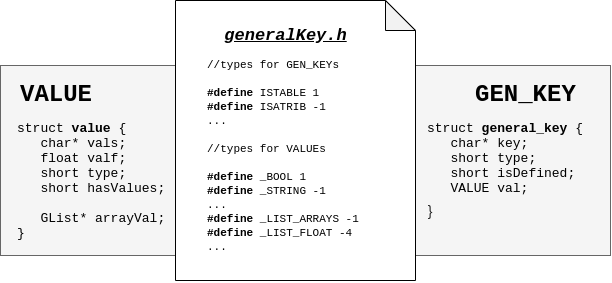
\includegraphics[scale=0.5]{images/PL_TP2_Structures-P2.png}
    \caption{Estruturas de dados para chaves e valores.}
    \label{fig:my_label}
\end{figure}

O valor (\textbf{struct value}) da \textit{struct general\_key} é novamente uma estrutura dada a variedade de informação que pode estar atribuída a uma chave, tendo para isso definido um conjunto de \textit{macros} para saber que tipo de dados se encontra armazenado na \textit{key}.
\par
Como se pode ver na figura anterior, todas estas estruturas e definições globais encontram-se definidas no \textit{header} \textbf{generalKey.h} para facilitar a organização do código C.
\par
As \textit{macros} presentes no caso das \textbf{GEN\_KEY} permitem perceber se a chave pode ter mais associações (\textit{values})
 ou não após terem sido criadas, ou seja, caso uma chave tenha um \textit{type} definido como \textit{ISTABLE} podemos deduzir que não existem valores associados a essa chave diretamente, isto é, apenas pode ter outras chaves filho no campo \textit{value} da \textit{hashtable}.
\par
Já a \textit{struct value} armazena o valor associado a uma dada \textit{key} após uma atribuição, podendo esse valor ser uma \textit{string}, um \textit{float} ou até um \textit{array} de valores.

\subsection{Exemplo de aplicação}

De forma simples, nesta secção, pretende-se mostrar o resultado esperado de um exemplo da linguagem \textbf{TOML} e o resultado esperado para a estrutura final de dados obtida:

\begin{figure}[h!]
    \centering
    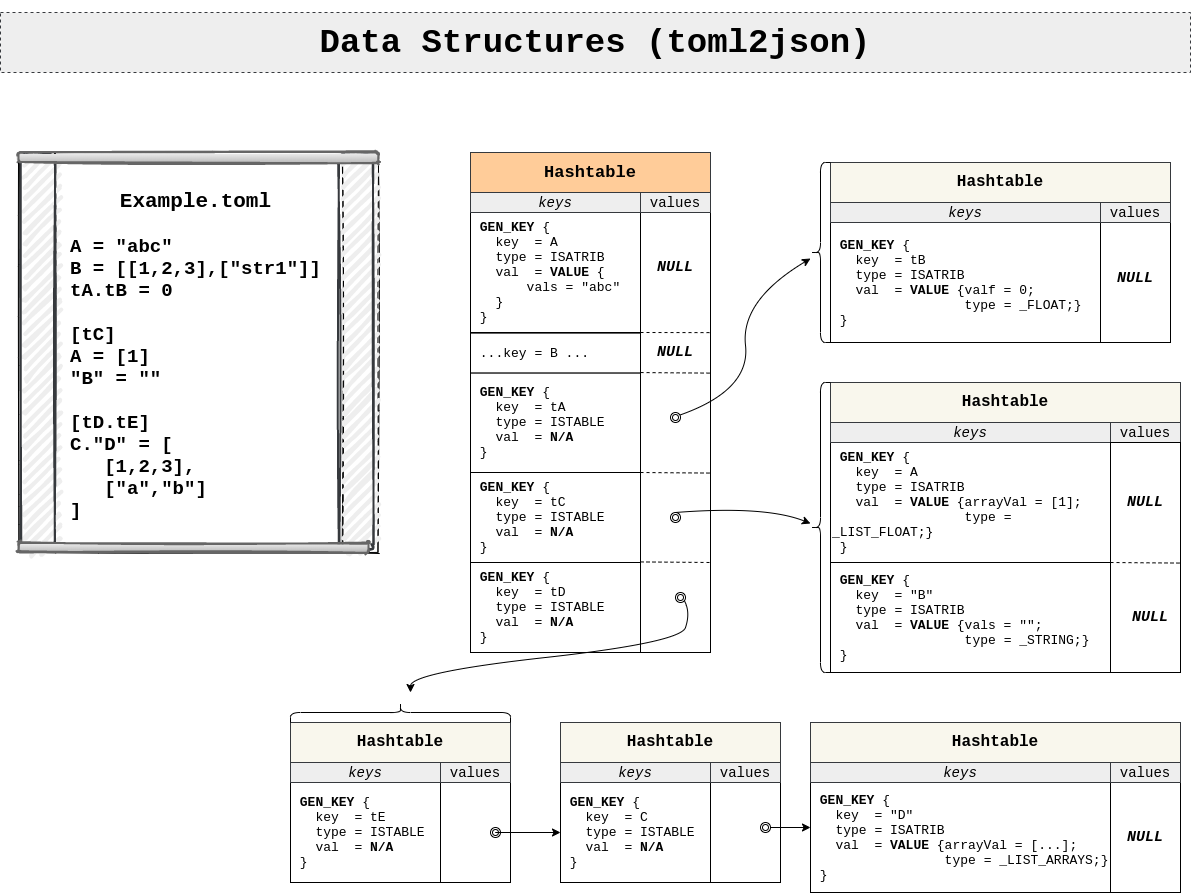
\includegraphics[scale = 0.36]{images/PL_TP2_Structures_1.png}
    \caption{Exemplo de aplicação TOML e estrutura final.}
    \label{fig:my_label}
\end{figure}

Este exemplo cobre, assim, grande parte dos casos válidos para definição de pares chave-valor neste trabalho, pelo que o a tabela final, representada à direita é sucessivamente criada à medida que o analisador sintático faz a leitura e aplicação de algoritmos de \textit{parsing bottom-up}.
\par
Numa próxima secção iremos abordar, de forma breve, como é feita a gestão desta tabela de \textit{hashing} ao nível das adições, controlo de valores duplicados e construção recursiva de tabelas.

\chapter{Estrutura do código}

\section{Árvore de ficheiros e código fonte}

A organização do código do programa final é uma parte importante para qualquer programa pelo que não foi ignorada de todo. Temos vários módulos em C com referência a diferentes porções de funções, estruturas e macros utilizadas em várias situações durante a análise sintática do \textbf{Yacc}.
\par
Os diferentes ficheiros que compõem o nosso trabalho seguem a seguinte estrutura em árvore:
\par


\begin{figure}[h!]
    \centering
    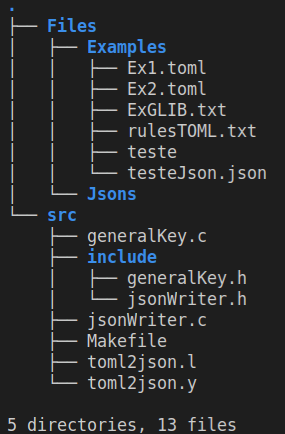
\includegraphics[scale=0.4]{images/Project-Tree-Folders.png}
    \caption{Árvore da diretoria raiz do projeto.                              }
    \label{fig:my_label}
\end{figure}

Na diretoria \textit{Files} temos diversos exemplos de aplicação de \textbf{TOML} que fomos obtendo da pesquisa que foi feita sobre o que se pode e não pode fazer nesta linguagem, assim como alguns \textit{inputs} exemplo ao programa, como o \textit{Ex1.toml}, enquanto que na diretoria \textit{Jsons} ficarão todos os \textit{outputs} do \textit{parser} no formato pretendido.
\par
Por outro lado, foram estabelecidos os \textit{headers} e os ficheiros relativos ao código fonte do projeto, armazenados na diretoria \textit{src}.
\par
Existem, portanto, dois ficheiros principais, o analisador léxico com o código do \textbf{FLex} \textit{toml2json.l} e o analisador sintático com o código do \textbf{Yacc} \textit{toml2json.y} onde é feito o reconhecimento de todos os símbolos terminais e onde são aplicadas as regras sintáticas manipulando esses \textit{tokens}.
\par
No módulo \textit{generalKey.c} definimos as várias funções que fazem a manipulação dos dados da estrutura final que será convertida para o formato pretendido e também a definição da estrutura das chaves e valores no respetivo \textit{generalKey.h}.
\par
Por fim, o \textit{jsonWriter.c} pretende encapsular as funções relativas à conversão dos dados das tabelas de \textit{hashing} definidas para o ficheiro \textit{output} final segundo as regras impostas por estruturas como o \textbf{JSON}.

\section{Construção das tabelas de \textit{hashing}}

Aproveitamos esta secção para descrever, de forma geral, como é feita a inserção e verificação de erros durante o processo de construção das tabelas que servirão de conversão dos dados para o formato final.
\par
A inserção de novas tabelas à estrutura de dados principal é um processo que deve ser feito verificando a existência de chaves já definidas que podem produzir o mesmo \textit{hash} e, por isso, substituir o valor anteriormente associado a uma determinada chave.
\par
Deste modo, quando é reconhecida uma nova chave, através da seguinte semântica:
\begin{verbatim}
    Hipótese 1: [chave1] # definir uma tabela indexada com chave1
    Hipótese 2: [chave1.chave2] # definir duas tabelas encadeadas
\end{verbatim}

É necessário verificar, deste modo, a existência de duplicados e isso é feito através da seguinte função, dado o seu protótipo \textbf{update\_table(tableEntrada, tabelaFinal)}.
\par
O algoritmo, de forma geral, recebe uma tabela de entrada, que corresponde à última tabela definida em \textbf{TOML} através das hipóteses especificadas acima, correspondendo também ao fim de processamento do símbolo não terminal: 
\begin{verbatim}
    Table : '[' TermTable ']' 
          ;
\end{verbatim}
Onde, após reconhecimento do \textit{TermTable}, o valor de \textbf{\$2} contém um encadeamento de \textit{GHashTable}s\footnote{Utilizaremos HT como abreviação para \textit{GHashTables} da \textbf{glib}.} com o termo a ser inserido, por exemplo:
\begin{verbatim}
    Exemplo 1: Inserir [chave1] produz a seguinte HT:
        $2 = (HT: key (chave1)) -> NULL
    Exemplo 2: Inserir [chave1.chave2] produz a seguinte HT:
        $2 = (HT: key (chave1)) -> (HT: key (chave2)) -> NULL
\end{verbatim}

A função introduzida acima tem então o trabalho de verificar se na HT \textbf{tabelaFinal} existe um encadeamento de HTs tal que corresponda ao caminho (\textit{path}) produzido pelos exemplos acima, caso exista deve reportar erro \textbf{-1} para as demais funções que a chamam.
\par
A função deve ser capaz então de verificar situações como:
\begin{verbatim}
    # inserir encadeamento a -> b -> c -> NULL
    # apenas a tabela "c" se encontra definida! "a" e "b" são (Not defined)
    [a.b.c]
    atribsC = ...
    
    # inserir, de seguida, "a" deve ser possível, mudando o seu estado
    # de (Not Defined) para (Defined)
    [a] 
    atribsA = ...
\end{verbatim}

\vspace{5cm}

\par A nível de atribuições foi necessário implementar funções capazes de atribuir \textit{values} a certos termos capazes de os suportar, ou seja, que fossem do tipo \textit{IS\_ATRIB}.
\par Para isso, a função \textbf{add\_lastTable} serviu como atualização do \textit{value} do term e consequente inserção no local correto da tabela final.
\begin{verbatim}
    Atrib : Term '=' Value
    # É sempre chamado o add_lastTable(...) de forma a inserir o
    Value no Term
\end{verbatim}  

\par Para a inserção ocorrer da forma esperada, é importante que o símbolo não terminal \textbf{Value} resolva e retorne o valor correto para a inserção.

\chapter{Resultados obtidos}

De forma a verificar os resultados do nosso conversor, foram desenvolvidos dois exemplos de ficheiros \textbf{TOML} a que o nosso programa consegue dar resposta, sendo que um deles é o disponibilizado pela equipa docente.
\par Para além de escrever a conversão num ficheiro previamente identificado, o conversor indica no terminal durante o tempo de execução as tabelas por ele lidas como forma de \textit{debug} e de perceber como ficará o resultado final.


\begin{figure}[H]
    \centering
    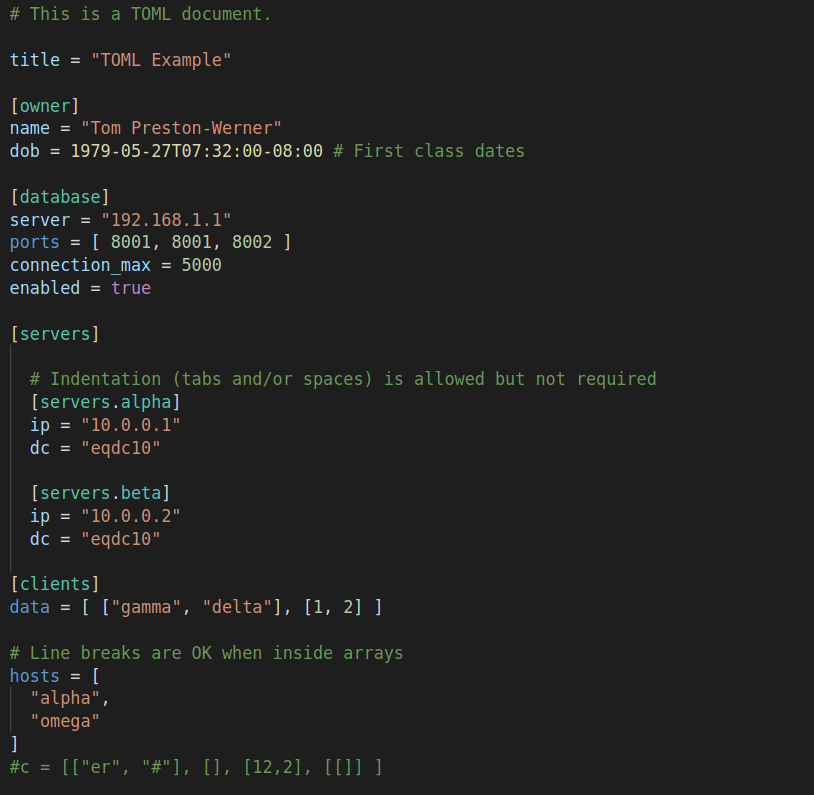
\includegraphics[scale = 0.4]{images/Ficheiro Toml.png}
    \caption{Ficheiro TOML}
    \label{fig:my_label}
\end{figure}


\par Assim, podemos ver de seguida um exemplo de aplicação do nosso conversor ao ficheiro \textbf{TOML} indicado em cima, dando o resultado final e alguns \textit{prints} durante a execução deste da nossa estrutura de dados.




\begin{figure}[H]
\centering
\begin{subfigure}
  \centering
  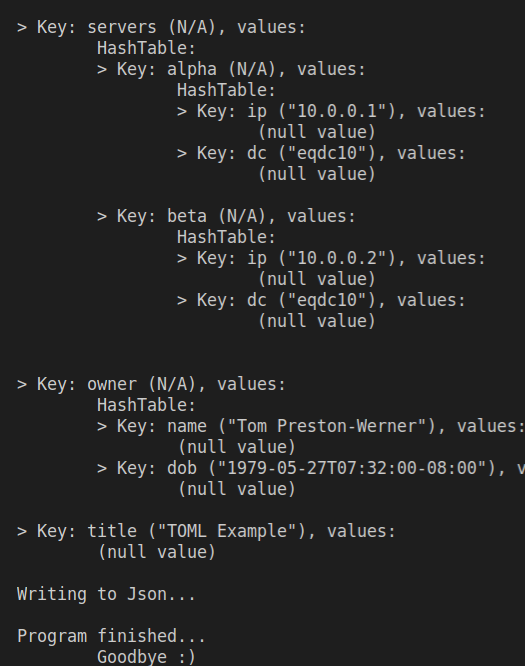
\includegraphics[width=.45\linewidth]{images/Prints em Exec.png}
  \label{fig:sub1}
\end{subfigure}
\begin{subfigure}
  \centering
  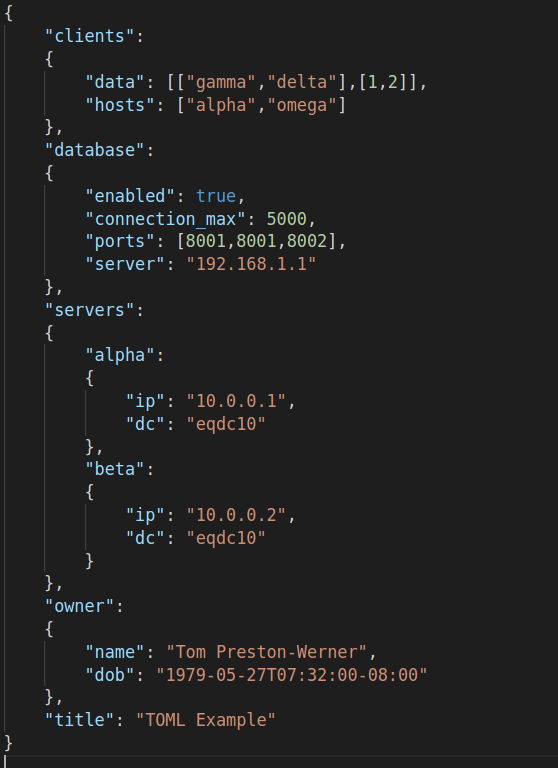
\includegraphics[width=.45\linewidth]{images/Json final Ex1.png}
  \label{fig:sub2}
\end{subfigure}
\caption{Estrutura de dados durante a execução e resultado final em JSON}
\label{fig:test}
\end{figure}

\par A imagem à esquerda representa os \textit{prints} durante o tempo de execução da nossa estrutura de dados, enquanto que a imagem à direita é o resultado da conversão do \textbf{TOML} para \textbf{JSON}.
\par De notar que o nosso conversor pode ser executado através do comando:

\begin{verbatim}
        make run < ../Files/Examples/Ex1.toml
\end{verbatim}



\chapter{Conclusão}

Este trabalho vem complementar a componente teórico-prática fortemente aplicada nesta unidade curricular pelo que serve de um bom teste aos nossos conhecimentos e a forma como podemos lidar com aquilo que é tão básico para um programador como um compilador.
\par
O trabalho em questão foi interessante no sentido em que pusemos em prática conhecimentos relativos a analisadores léxicos como o \textbf{FLex} e à importância do mesmo no que toca ao processo de \textit{parsing} e deteção de caracteres de erro para uma linguagem, analisadores sintáticos como o \textbf{Yacc} resolvendo por vezes conflitos relativos aos algoritmos de \textit{parsing bottom-up} e a estratégias para os resolver e também outras linguagens de programação como o \textbf{TOML} que são usualmente preferidas em situações de configuração de programas e dispositivos simples. 
\par
Por outro lado, a aplicação de algoritmos em estruturas de dados complexas serviu de revisão e reforço da sua importância no desenvolvimento de compiladores rápidos e eficientes, reutilizando APIs públicas do C na aplicação prática dos mesmos.
\par Em suma, achamos que este trabalho teve grande proveito no que toca ao assimilar de conhecimentos relativos ao desenvolvimento de \textit{Processadores de Linguagens Regulares} que filtram e transformam textos, identificando semânticas, tendo em base o conceito de regras de produção \textit{Condição-Ação} e, a nosso ver, cumprimos os requisitos propostos pela equipa docente no que toca a este projeto.


\end{document}











